\documentclass[../main.tex]{subfiles}

\begin{document}
	\subsection{NAND2 transfer function}
	{
	
	\begin{figure}[H]
		\centering
		\begin{circuitikz}
			% PMOS Transistors (Pull-up Network)
			\node[pmos, anchor=D] (P1) at (0,0) {};
			\node[pmos, anchor=D] (P2) at (2,0) {};
			
			% NMOS Transistors (Pull-down Network)
			\node[nmos, anchor=D] (N1) at (1,-0.5) {};
			\node[nmos, anchor=D] (N2) at (1,-1.5) {};
			
			% Output Line
			\draw (P1.D) -- (P2.D) -- (3,0) node[right]{$V_{out}$};
			
			% PMOS Connections
			\draw (P1.S) -- ++(0,0.5) node[above]{$V_{DD}$}; % P1 drain to VDD
			\draw (P2.S) -- ++(0,0.5) node[above]{$V_{DD}$}; % P2 drain to VDD
			
			% NMOS Connections
			\draw (N2.S) -- ++(0,-0.5) node[ground, below]{};     % N1 source to GND
			\draw (N1.S) -- (N2.D);                          % N1 drain to N2 source
			\draw (N1.D) -- (1,0);                           % N2 drain to output
			
			% Input Connections
			\draw (P1.G) -- ++(-0.4,0) node[left]{$A$};        % A to P1 gate
			\draw (N1.G) -- ++(-0.4,0) node[left]{$A$};        % A to N1 gate
			\draw (P2.G) -- ++(-0.4,0) node[left]{$B$};        % B to P2 gate
			\draw (N2.G) -- ++(-0.4,0) node[left]{$B$};        % B to N2 gate
		\end{circuitikz}
	\end{figure}
		
	\begin{tcolorbox}[colback=gray!5!white,colframe=gray!75!black]
		Plot the static transfer function of the NAND2 gate in the following cases:
		\begin{itemize}
			\item The entries $A$ and $B$ of this NAND gate are connected to the same input signal which varies from $V_{SS}$ to $V_{DD}$. In this scenario the two inputs switch at the same time.
			\item The $A$ input is at high state (voltage $V_{DD}$), and the $B$ voltage varies from $V_{SS}$ to $V_{DD}$. This corresponds to commutations which do not occur at the same time.
		\end{itemize}
		Deduce the noise margin on the input low state and high state.
	\end{tcolorbox}
	
	\subsubsection{Simultaneous switch}
	{
		
		We observe that $A = B = 0 \implies \bar{A \cdot B} = 1$ and $A = B = 1 \implies \bar{A \cdot B} = 0$. Thus, we expect the output graphic to look like an inverter and we can compute the margins like we did in the previous question.
		
		\begin{lstlisting}
			.include cmosws.mod
			
			Vdd 1 0 dc 3.3V
			Vin 2 0 dc 1.0V
			M1  1 2 4 1 MODP L=0.6U W=6.0U
			M2  1 2 4 1 MODP L=0.6U W=6.0U
			M3  4 2 5 0 MODN L=0.6U W=6.0U
			M4  5 2 0 0 MODN L=0.6U W=6.0U
			
			.dc Vin 0 3.3 50mV
			.end
		\end{lstlisting}
		
		\begin{figure}[H]
			\centering
			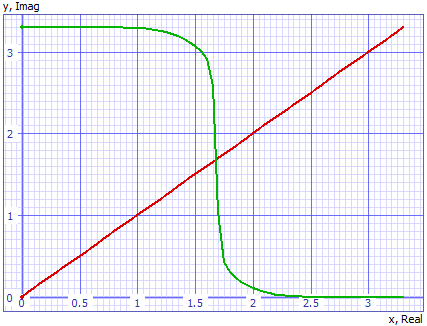
\includegraphics[width=0.5\textwidth]{plots/Q5_1.png}
			\caption{In red, we have inputs A and B. In green the output of the NAND2 gate.}
		\end{figure}
		
		We get from the graphic
		
		\begin{itemize}
			\item $V_{IL} = 0,97$V (maximum $A,B$ for which $V_{out}$ is high)
			\item $V_{IH} = 2,32$V (minimum $A,B$ for which $V_{out}$ is low)
			\item again we consider $V_{OL} = 0$V and $V_{OH} = 3,3$V.
		\end{itemize}
		
		We conclude that
		\begin{itemize}
			\item $NML = V_{IL} - V_{OL} = 0,97$V
			\item $NMH = V_{OH} - V_{IH} = 3,3 - 2,32 = 0,98$V
		\end{itemize}
	}
	
	\subsubsection{Non-simultaneous switch}
	{
		Now we fix $A = 1$. For $B=0$, we have $\bar{A \cdot B} = 1$ and for $B = 1$, we have $\bar{A \cdot B} = 0$. Thus, if we consider $V_{in} = B$ we have once again an inverter and we can compute the margins like we did previously.
		
		\begin{lstlisting}
			.include cmosws.mod
			
			Vdd 1 0 dc 3.3V
			Va  2 0 dc 3.3V
			Vb  3 0 dc 1.0V
			M1  1 2 4 1 MODP L=0.6U W=6.0U
			M2  1 3 4 1 MODP L=0.6U W=6.0U
			M3  4 2 5 0 MODN L=0.6U W=6.0U
			M4  5 3 0 0 MODN L=0.6U W=6.0U
			
			.dc Vb 0 3.3 50mV
			.end
		\end{lstlisting}
		
		\begin{figure}[H]
			\centering
			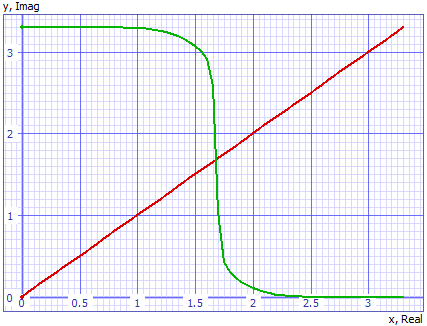
\includegraphics[width=0.5\textwidth]{plots/Q5_1.png}
			\caption{In red, we have input B. In green the output of the NAND2 gate.}
		\end{figure}
		
		We get from the graphic
		
		\begin{itemize}
			\item $V_{IL} = 0,87$V (maximum $A,B$ for which $V_{out}$ is high)
			\item $V_{IH} = 2,31$V (minimum $A,B$ for which $V_{out}$ is low)
			\item again we consider $V_{OL} = 0$V and $V_{OH} = 3,3$V.
		\end{itemize}
		
		We conclude that
		\begin{itemize}
			\item $NML = V_{IL} - V_{OL} = 0,87$V
			\item $NMH = V_{OH} - V_{IH} = 3,3 - 2,31 = 0,99$V
		\end{itemize}
		
		Comparing the margins calculated, we conclude that the simultaneous switch gives a more centered curve.
	}
	
	}
\end{document}